\Chapter{STUDENT MODELLING METHODS}\label{sec:RevLitt}

A large body of methods have been developed for student modeling. They are used to represent and assess student skills and they are a fundamental part of intelligent learning environments \citep{Desmarais2011}. These models have been proposed both for dynamic performance data, where a time dimension is involved and where a learning process occurs (see for eg. Bayesian Knowledge Tracing in \citet{Koedinger2011}), and for static performance data where we assume student skill mastery is stationary. In this thesis, we focus on static performance data.


We assume that skills explain the performance and test outcome prediction. Student models incorporate single or multiple skills. Some even model performance without explicit skills and we will refer to them as zero-skill models. The most widely used one is Item Response Theory (IRT). In its simplest version, IRT considers a single skill for student performance data. Of course, sometimes there are many skills involve in a single problem and therefore this model becomes insufficient for many applications in Intelligent Tutoring Systems (ITS). Under certain conditions, multi-skills models can perform better in that case. Other methods, such as POKS, have no latent skills. They just look at the relation between those items that are directly observable among test outcome items. The details of each category of techniques along with some examples are described in the next section.

\section{Definitions and concepts}

In this section some concepts and basic definitions that are common between most of student models are described. 
 
\subsection{Test outcome data}

The student test outcome data, or more simply student test data, can consist in results from exams or from exercises, in the context of an e-learning environment or in paper and pencil form. We use the term \textit{item} to represent exercises, questions, or any task where the student has to apply a skilled performance to accomplish. Student answers are evaluated and categorized as success~(1) or failure~(0). The data represents a snapshot of the mastery of a student for a given subject matter, as we assume that the student's knowledge state has not changed from the time of answer to the first question item to the last one.

Test data is defined as an $m \times n$ matrix, $\mathbf{R}$. It is composed of $m$~row items and $n$~column students. If a student successfully answers an item, the corresponding value in the results matrix is 1, otherwise it is 0.

\subsection{Skills}

In this thesis we consider skills as problem solving abilities. For example in mathematics ``addition'', ``division'' are typical skills. They can also be further detailed, such as single digit and multi-digit addition. There may be a single skill required to solve a problem or multiple skills. Skills are termed \textit{latent} because they are never observed directly.

If an item requires multiple skills, there are three different ways in which each skill can contribute to succeed a problem: The first case is when mastering a skill is mandatory for a student to succeed an item that requires it. The second case is when the skill increases the chance to succeed a problem. The third case is when at least one of the skills from the set of skills for an item is required to succeed that item. We will see later that the temrs \textit{conjunctive}, \textit{compensatory}/\textit{additive}, and \textit{disjunctive} are often used to refer to each case respectively.

Skills can have different range of values based on the student model definition. For example, the single skill in IRT is continuous in $\mathbb{R}$ and typically ranges between~$-4$ to~$+4$. Some student models consider skills range between~$0$ and~$1$. Finally, other models have binary~$1$ or~$0$ skills, which means it can be mastered or not. Details of definition of skills for each student model are given later in this chapter.

\subsection{Q-matrix and Skill mastery matrices}


Curriculum design can be a complex task and an expert blind spots in designing curricula is possible. It is desirable to have an alternative to human sequenced curricula. To do so, there should be a model designed for this purpose which maps skills to items \citep{Tatsuoka1983,Tatsuoka2009}. Figure~\ref{QItemInt} shows an example of this mapping which is named Q-matrix. Figure~\ref{ItemInt} shows 4 items and each item requires different skills (or combination of skills) to be successfully answered. Assuming 3 skills such as fraction multiplication ($s_{1}$), fraction addition ($s_{2}$) and fraction reduction ($s_{3}$), these questions can be mapped to skills like the Q-matrix represented in figure~\protect\ref{QInt}. 

Such a mapping is desirable and very important in student modeling; because optimal order of problems (sequence of repetition and presentation) can be determined by this model since it allows prediction of which item will cause learning of skills that transfer to the other items most efficiently. It can also be used to assess student knowledge of each concept, and to personalize the tutoring process according to what the student knows or does not know. For example, Heffernan et al. in \citep{feng2009using} have developed an intelligent tutoring system (the ASSISTment system) that relies on fine grain skills mapped to items. Barnes, Bitzer, \& Vouk in \citep{barnes2005experimental} were among the early researchers to propose algorithms for automatically discovering a Q-Matrix from data. In some context there is a constraint for the number of latent skills which is: $k<nm/(n+m)$ \protect\citep{lee1999learning} where $k$ , $n$ and $m$ are number of skills, students and items respectively.

\begin{footnotesize}
\begin{figure}[h]
\centering

\subfigure[Skills]{
   $\begin{array}{cl}
   &\\
   &\\
   s_{1} : & \text{fraction multiplication}\\
   &\\
   s_{2} : & \text{fraction addition}\\
   &\\
   s_{3} : & \text{fraction reduction}\\
   &\\
   &
\end{array}$
}
\quad
\subfigure[Items with different skills]{
   $\begin{array}{cc}
i_{1} & \frac{4}{\frac{12}{3}}+\frac{3}{5}=\frac{8}{5}\\
 &  \\
i_{2} & \frac{4}{\frac{12}{3}}=\frac{4{\times}3}{12}=\frac{12}{12}=1\\
 &  \\
i_{3} & 1+\frac{3}{5}=\frac{8}{5}\\
 &  \\
i_{4} & 2{\times}\frac{1}{2}=1\\
&
\end{array}$
\label{ItemInt}
}
\quad
 \subfigure[Q-matrix]{

$\begin{array}{c}
\begin{array}{cc}
 & \textrm{Skills}\\
 & \begin{array}{ccc}
s_{1} & s_{2} & s_{3}\end{array}\\
\mathrm{\begin{sideways}Items\end{sideways}}\begin{array}{c}
i_{1}\\
i_{2}\\
i_{3}\\
i_{4}
\end{array} & \left[\begin{array}{ccc}
1 & 1 & 1\\
1 & 0 & 1\\
0 & 1 & 1\\
1 & 0 & 1
\end{array}\right]
\end{array}\\
\\
\\

\end{array}$
\label{QInt}
}
\caption{Four items and their corresponding Q-matrix}\label{QItemInt}
\end{figure}
\end{footnotesize}

The skills mastery matrix, \textbf{S}, represents student skills mastery profiles. In this matrix rows are skills and columns represent examinees. A cell with the value of 1 in $\mathbf{S}_{ij}$ indicates that examinee $j$ is proficient in skill $i$ and a value of 0 shows that he does not have the related skill.



\subsection{Types of Q-matrices}
 
As explained earlier, skills can have three interpretations when they contribute to succeed an item. These interpretations can be reflected in Q-matrices. There exists three different types of Q-matrices which are useful based on the context of a problem domain:

\begin{itemize}
\item \textbf{Conjunctive}: The most common one is the conjunctive model of the Q-matrix which is the standard interpretation of the Q-matrix in Educational Data Mining. In this type, a student should master all the required skills by an item to succeed it. If a student misses any one of these skills, then the result will be a failure in the test outcome data. Thus there is a conjunction between required skills.

\item \textbf{Additive} (compensatory): Compensatory or additive model of skills is an interpretation of a Q-matrix where each skill contributes some weight to succeed that item. For example, if an item requires two skills $a$ and $b$ with the same weight for each of them, then each skill will contribute equally to yield a success of the item. In the compensatory model of Q-matrix, each skill increases the chance of success based on its weight.

\item \textbf{Disjunctive}: In the disjunctive model, mastery of any single skill required by an item is sufficient in order to succeed the related item.
\end{itemize}

Note that in practice these types of interpretations becomes reasonable when there is at least one item in the Q-matrix that requires more than one skill otherwise they preform the same as each other. Later in this chapter these types will be described in more details with examples.


Q-matrices can also be categorized according to the number of skills per item:
\begin{itemize}
\item Single skill per item: Each item should have exactly one skill but the Q-matrix can have many skills.
\item Multiple skills per item: Any combination of skills with at least one skill is possible for items.
\end{itemize}

\section{Skills assessment and item outcome prediction techniques}
\label{SkillsAssessmentModels}

The skills assessment models we compare can be grouped into four categories: (1) the Knowledge Space frameworks which models a knowledge state as a set of observable items without explicit reference to latent skills, (2) the single skill Item Response Theory (IRT) approach, (3) the matrix factorization approach, which decomposes the student results matrix into a Q-matrix that maps items to skills, and a skills matrix that maps skill to students, and which relies on standard matrix algebra for parameter estimation and item outcome prediction, and finally (4) the DINA/DINO approaches which also refer to a Q-matrix, but incorporate slip and guess factors and rely on different parameter estimation techniques than the matrix factorization method. We focus here on the assessment of static skills, where we assume the test data represents a snapshot in time, as opposed to models that allow the representation of skills that change in time, which is more typical of data from learning environments (see \citet{desmarais2012review}, for a review of both approaches).



The skills assessment model we compare can be classified at a first level according to whether they model skills directly, and whether they are single or multiple skills. Then, multi-skills model can be further broken down based on whether they have guess and slip parameters, and whether the skills are considered disjunctive or conjunctive. Figure~\ref{AssessMethods} shows this hierarchy of models.

\begin{figure}[ht]
\centering
   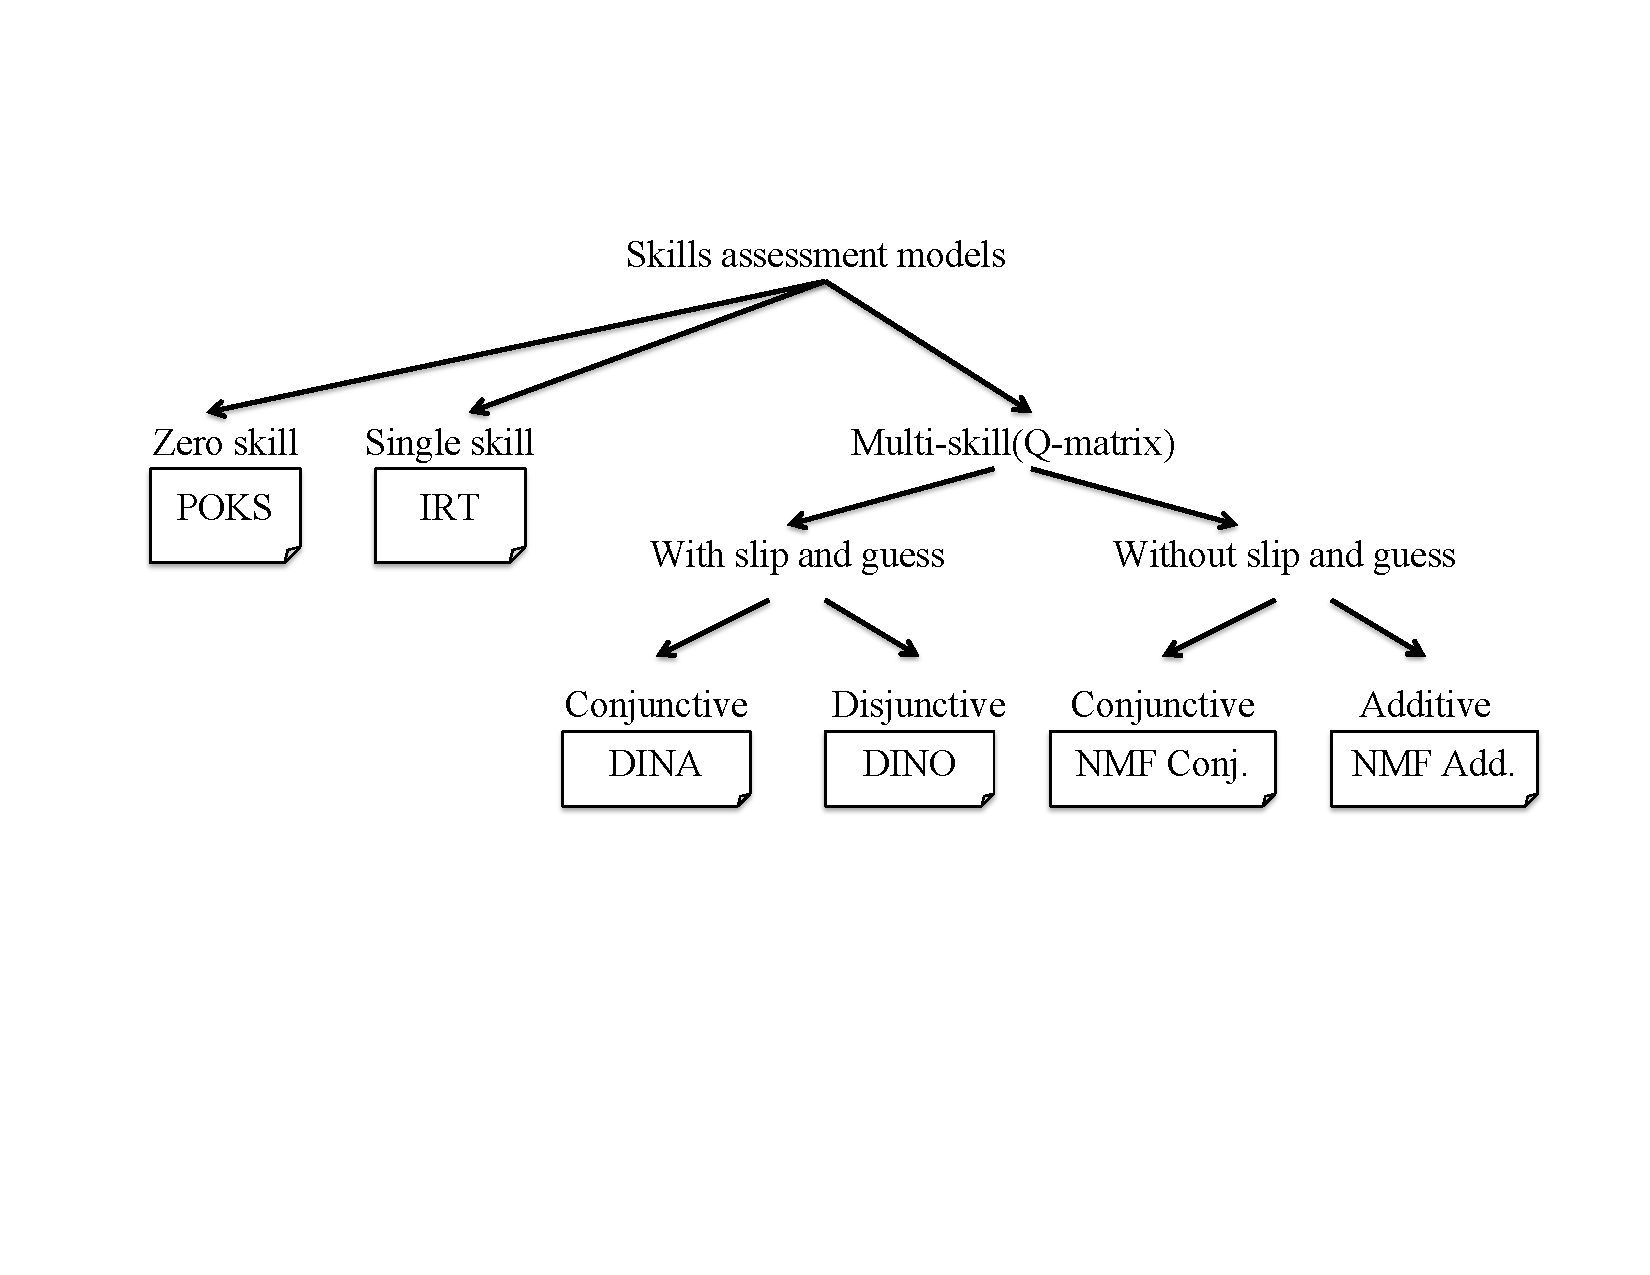
\includegraphics[trim=0.5cm 7cm 0.5cm 3cm,scale =0.5] {SkillsAssessments.pdf}
\caption{Skills assessment methods}
\label{AssessMethods}
\end{figure}

Considering these techniques from the perspective of variety of skills in test outcome prediction, we can put them in the following categories: 

\begin{itemize}

\item Zero skill technique that predict item outcome based on observed items. POKS is the technique that is used from this category.
\item Single skill approaches, where every item is linked to the same single skill. Item Response Theory (IRT) is the typical representative of this approach, but we also use the ``expected value'' approach which, akin to IRT, incorporates estimates of a the student's general skill and the item difficulty to yield a predicted item outcome.
\item Multi-Skills techniques that rely on Q-matrices to predict test outcome. Deterministic Input Noisy And/Or (DINA/DINO), NMF Conjunctive and \ac{NMF} additive are the techniques we use in this study.

\end{itemize}  
Note that the ``expected value'' approach is also considered as a baseline for our evaluations. 

The details of the different approaches are described below.

\section{Zero skill techniques}

\textit{Zero skill techniques} are so called because they make no explicit reference to latent skills. They are based on the Knowledge Space theory of Doignon and Falmagne \citep{Doignon1999,desmarais:umuai:2006}, which does not directly attempt to model underlying skills but instead rely on observable items only. An individual's knowledge state is represented as a subset of these items. In place of representing skills mastery directly, they leave the skills assessment to be based on the set of observed and predicted item outcomes which can be done in a subsequent phase. TETRAD \citep{scheines1998tetrad} is a software that identifies pre-requisite relationships among items which is widely used in EDM.

POKS is one of the models adopted in our study that is a derivative of Knowledge Space Theory. POKS stands for Partial Order Knowledge Structures. It is a more constrained version of Knowledge Spaces theory \citep{desmarais:umuai:1995}. POKS assumes that items are learned in a strict partial order. It uses this order to infer that the success to hard items increases the probability of success to easier ones, or conversely, that the failure to easy items decreases the chances of success to harder ones.

\subsection{Knowledge Spaces and Partial Order Knowledge Structures (POKS)}
\label{POKS-Lit-Rev}
Items are generally learnt in a given order. Children learn easy problems first, then harder problems. It reflects the order of learning a set of items in the same problem domain. POKS learns the order structure from test data in a probabilistic framework. For example in figure \ref{fig2} four items are shown in a partial order of knowledge structure. It is required for an examinee to be able to answer $i_{4}$ in order to solve $i_{3}$ and $i_{2}$. Also for solving $i_{1}$, one should be able to answer $i_{2}$, $i_{3}$ and $i_{4}$. if an examinee was not able to answer $i_{4}$ then he would have less chance to answer correctly other items.

\begin{figure}[h]
\begin{footnotesize} \begin{diagram}[notextflow]    & & i_{1}:\frac{4}{\frac{12}{3}}+\frac{3}{5}=\frac{8}{5} & &   \\    & \ldTo_a & & \rdTo_b &   \\    & & & &   \\   i_{2}:\frac{4}{\frac{12}{3}}=\frac{4{\times}3}{12}=\frac{12}{12}=1 & & & & i_{3}:1+\frac{3}{5}=\frac{8}{5}  \\    & & & &   \\    & \rdTo_c & & \ldTo_d &   \\    & & i_{4}:2{\times}\frac{1}{2}=1 & &    \\  \end{diagram} \end{footnotesize}

\caption{Partial Order Structure of 4 items}

\label{fig2} 
\end{figure}

This is reflected in the results matrix $\mathbf{R}$ by closure constraints on the possible knowledge states. Defining a student knowledge state as a subset of all items (i.e. a column vector in $\mathbf{R}$), then the space of valid knowledge states is closed under union and intersection according to the theory of Knowledge spaces \citep{Doignon1985}. In POKS, this constraint is relaxed to a closure under union, meaning that the union of any two individual knowledge states is also a valid knowledge state. This means that the constraints can be expressed as a partial order of implications among items, termed a Partial Order Knowledge Structure (POKS). The algorithm to derive such structures from the data in $\mathbf{R}$ relies on statistical tests \citep{desmarais:umuai:1996,desmarais:2005}.

A knowledge structure can be represented by an Oriented incidence matrix, O, or by an Adjacency matrix, A. In the oriented incidence matrix, rows are edges and columns are nodes of the graph. The value of -1 shows the start node of an edge and 1 indicates the end of an edge. Therefore for each row (edge) there is only one pair of (-1,1) and the rest of cells are 0. In adjacency matrix both rows and columns are Items and if there is a link between a pair of items (for example $i\rightarrow j$) there should be a 1 in $A_{ij}$ otherwise it is 0. Figure \ref{fig3IMAM} shows the corresponding oriented incidence matrix and adjacency matrix of the structure in figure~\ref{fig2}. 


\begin{figure}[h]
\[
\begin{array}{ccccc}
\begin{array}{cc}
 & \begin{array}{cccc}
i_{1} & i_{2} & i_{3} & i_{4}\end{array}\\
\begin{array}{c}
a\\
b\\
c\\
d
\end{array} & \left(\begin{array}{cccc}
-1 & 1 & 0 & 0\\
-1 & 0 & 1 & 0\\
0 & -1 & 0 & 1\\
0 & 0 & -1 & 1
\end{array}\right)
\end{array} &  &  &  & \begin{array}{cc}
 & \begin{array}{cccc}
i_{1} & i_{2} & i_{3} & i_{4}\end{array}\\
\begin{array}{c}
i_{1}\\
i_{2}\\
i_{3}\\
i_{4}
\end{array} & \left(\begin{array}{cccc}
0 & 1 & 1 & 0\\
0 & 0 & 0 & 1\\
0 & 0 & 0 & 1\\
0 & 0 & 0 & 0
\end{array}\right)
\end{array}\\
\\
\\
O &  &  &  & A
\end{array}
\]


\caption{Oriented incidence matrix and Adjacency matrix}
\label{fig3IMAM}
\end{figure}


The structure of the partial order of items is obtained from a statistical hypothesis test that reckons the existence of a link between two items, say $A \rightarrow B$, on the basis of two Binomial statistical tests $P(B|A) > \alpha_1$ and $P(\neg A|\neg B) > \alpha_1$ and under a predetermined alpha error of an interaction test ($\alpha_2$). The $\chi^2$ test is often used, or the Fisher exact test. The values of $\alpha_1 = .85$ and $\alpha_2 = .10$ are chosen in this study across all experiments.

A student knowledge state is represented as a vector of probabilities, one per item. Probabilities are updated under a Naive Bayes assumption as simple posterior probabilities given observed items.

Inference in the POKS framework to calculate the node's probability relies on standard Bayesian posteriors under the local independence assumption. The probability update for node $H$ given $E_1$,...~$E_n$ can be written in following posterior odds form:
\begin{equation}
O(H|E_1,E_2, ... , E_n) = O(H) \prod_{i}^{n} \frac{P(E_i|H)}{P(E_i | \overline{H})}
\label{EQPOKSratio}
\end{equation}
where odds definition is $O(H|E) = \frac{P(H|E)}{1-P(H|E)}$. If evidence $E_i$ is negative for observation $i$, then the ratio $\frac{P(\overline{E_i}|H)}{P(\overline{E_i}|\overline{H})}$ is used. \citet{desmarais:umuai:1996} provides more details on inference in POKS.


\section{Single skill approaches}

Other approaches incorporate a single latent skill in the model. This is obviously a strong simplification of the reality of skilled performance, but in practice it is a valid approximation as results show. When a model uses single latent skill, in fact it projects all the skills mastery level in a form of uni-dimensional representation that implicitly combines all skills. Then there would be a single continuous skill variable which is a weighted average of the skills mastery levels of an examinee. 

In this section two approaches for modeling static test data are presented: the well established Item Response Theory (IRT), which models the relationship between observation and skill variable based on a logistic regression framework. It dates back to the 1960's and is still one of the prevailing approaches \citep{bakerKim2004}. The second approach is a trivial approach we call \textbf{Expected Prediction}. This approach is also used as a baseline in our experiments.

\subsection{IRT} 

The \textbf{IRT family} is based on a logistic regression framework. It models a single latent skill (although variants exists for modeling multiple skills) \citep{bakerKim2004}. Each item has a difficulty and a discrimination parameter.

IRT assumes the probability of success to an item~$X_j$ by student $i$ is a function of a single ability factor~$\theta_i$: 
\[P(X_j\!=\!1\;|\;\theta_i) = \frac{1}{1+e^{-a_j(\theta_i-b_j)}}\]
In the two parameter form above, referred to as IRT-2pl, where parameters are:

\begin{itemize}
\item[$a_j$] represents the item discrimination;
\item [$b_j$] represents the item difficulty, and
\item [$\theta_i$] the ability of a single student.
\end{itemize}

Student ability, $\theta_i$, is estimated by maximizing the likelihood of the observed response outcomes probabilities:
\[ P(X_1, X_2, ..., X_j, \theta_i) = \prod_j P(X_j|\theta_i) \]
This corresponds to the usual logistic regression procedure. Note that the 2PL version of IRT is equivalent to the 3PL model with $c$ parameter equal to zero which represents pseudo guessing.

A simpler version of IRT called the Rash model, fixes the discrimination parameter,~$a$, to~$1$. Fixing this parameter reduces overfitting, as the discrimination can sometimes take unrealistically large values. Rash model is a valid model for student skills modeling, but we do use the more general IRT-2pl model, which includes both~$a$ and $b$, for the synthetic data generation process in order to make this data more realistic (chapter \ref{sec:Syn} discusses data generation approaches in details).

\subsection{Baseline Expected Prediction}\label{sec:basel-expect-pred}

As a baseline model, we use the expected value of success to item~$i$ by student~$j$, as defined by a product of odds:
\[ O(X_{ij}) =  O(X_i) O(S_j) \]
where $O(X_i)$ is the odds of success to item~$i$ by all participants and $O(S_j)$ is the odds of success rate of student~$j$. Both odds can be estimated from a sample. Recall that the transformation of odds to probability is $P(X) = 1/(1+O(X))$, and conversely $O(X) = P(X)/(1 - P(X))$. Probabilities are estimated using the Laplace correction: $P(X) = (f(x\!=\!1) + 1) / (f(x\!=\!1) + f(x\!=\!0) + 2)$, where $f(x=\{1,0\})$ represents the frequency of the corresponding category $x=1$ or $x=0$.


\section{Multi-skills techniques}
\label{NMF_DESC}
Finally the last category of student skills assessment models are considering student test result with multiple latent skills. Representation of multiple skills is possible in the form of a Q-matrix where skills are mapped to each item. As explained before, there exist different types of Q-matrices that each type represents a unique interpretation. The following sections will describe different skills assessment models along with their specific type of Q-matrix.


Still this category of models can be divided into two sub-categories: 
\begin{itemize}
\item Models that infer a Q-matrix from test result data, such as models that uses matrix factorization techniques.
\item Models that require a predefined Q-matrix to predict test outcome. These techniques can not directly infer the Q-matrix but they can refine an existing expert-defined Q-matrix.
\end{itemize}

Deriving a Q-matrix from a test result matrix is challenging. Some models require a pre-defined Q-matrix. In some cases an expert defined Q-matrix is available but minor mistakes in mapping skills to items are always possible even by an expert. The basic challenge is to derive a perfect Q-matrix out of a test result matrix to give it as an input parameter to some models. This challenge also creates other challenges such as optimum number of latent skills for a set of items in a test outcome. Sometimes there exist more than single Q-matrix associated with a test result with different number of skills. Finding the optimum number of skills to derive a Q-matrix is a question that is given in more details in section \ref{EDM2012}. 

Given the number of latent skills, there exist few techniques to derive a Q-matrix for models that require one. Cen et al. \citep{Cen2005,Cen2006} have used Learning Factor Analysis(LFA) technique to improve the initially hand-built Q-matrix which maps fine-grained skills to questions. They used log data which is based on the fact that the knowledge state of student dynamically changes over time as the student learns. In the case of static data of student knowledge, Barnes \citep{Barnes06} developed a method for this mapping which works based on a measure of the fit of a potential Q-matrix to the data. It was shown to be successful as well as Principal Component Analysis for skill clustering analysis. In our experiment we use NMF as a technique to derive a Q-matrix given an optimum number of latent skills. Later in this section we will introduce NMF in more details. Section \ref{ITS2012} describes how to derive a conjunctive model of Q-matrix from a student test result.

For real datasets there exists few expert defined Q-matrices. To use them as an input parameter for student skills assessment models we need to refine them. Section \ref{edm2014} gives few approaches to this problem.


\subsection{Types of Q-matrix (examples) }

As mentioned before, there are three models for the Q-matrix which are useful based on the context of the problem domain. The most important one is the conjunctive model of the Q-matrix, which is the standard interpretation of the Q-matrix. In figure \ref{fig1} an example of conjunctive model of Q-matrix is shown. Examinee $e_{1}$ answered item $i_{1}$ and item $i_{4}$ because he has mastered in the required skills but although he has skill $s_{1}$ he couldn't answer item $i_{3}$ which requires skill $s_{2}$ as well.

\begin{figure}[h]
\begin{footnotesize} 
\[
\begin{array}{ccc}
\begin{array}{cc}
 & \textrm{Examinee}\\
 & \begin{array}{cccc}
e_{1} & e_{2} & e_{3} & e_{4}\end{array}\\
\mathrm{\begin{sideways}Items\end{sideways}}\begin{array}{c}
i_{1}\\
i_{2}\\
i_{3}\\
i_{4}
\end{array} & \left[\begin{array}{cccc}
1 & 0 & 1 & 0\\
0 & 1 & 0 & 0\\
0 & 0 & 1 & 0\\
1 & 0 & 0 & 0
\end{array}\right]
\end{array} & \begin{array}{cc}
 & \textrm{Skills}\\
 & \begin{array}{ccc}
s_{1} & s_{2} & s_{3}\end{array}\\
\mathrm{\begin{sideways}Items\end{sideways}}\begin{array}{c}
i_{1}\\
i_{2}\\
i_{3}\\
i_{4}
\end{array} & \left[\begin{array}{ccc}
1 & 0 & 0\\
0 & 1 & 1\\
1 & 1 & 0\\
1 & 0 & 1
\end{array}\right]
\end{array} & \begin{array}{cc}
 & \textrm{Examinees}\\
 & \begin{array}{cccc}
e_{1} & e_{2} & e_{3} & e_{4}\end{array}\\
\mathrm{\begin{sideways}Skills\end{sideways}}\begin{array}{c}
s_{1}\\
s_{2}\\
s_{3}
\end{array} & \left[\begin{array}{cccc}
1 & 0 & 1 & 0\\
0 & 1 & 1 & 1\\
1 & 1 & 0 & 0
\end{array}\right]
\end{array}\\
\\
R & Q & S
\end{array}
\]
 \end{footnotesize} \caption{An example for Conjunctive model of Q-matrix}


\label{fig1} 
\end{figure}


The other type is the additive model of Q-matrix. Compensatory or additive model of skills is an interpretation of a Q-matrix where skills have weights to yield a success for that item. For example, considering an item that requires two skills $a$ and $b$ with the same weight each. Then each skill will contribute equally to yield a success of the item. In the compensatory model of Q-matrix, each skill increases the chance of success based on its weight. It is possible to have different weights for skills where skills for each item will sum up to~$1$. Figure \ref{fig1Add} represents an example of an additive model of Q-matrix with its corresponding result matrix. The value $R_{ij}$ can be considered as a probability that examinee $i$ can succeed item $j$.

\begin{figure}[h]
\begin{footnotesize} 
\[
\begin{array}{ccc}
\begin{array}{cc}
 & \textrm{Examinee}\\
 & \begin{array}{ccccccc}
e_{1} && e_{2} && e_{3} && e_{4}\end{array}\\
\mathrm{\begin{sideways}Items\end{sideways}}\begin{array}{c}
i_{1}\\
i_{2}\\
i_{3}\\
i_{4}
\end{array} & \left[\begin{array}{cccc}
1 & 0 & 1 & 0\\
0.5 & 1 & 0.5 & 0.5\\
0.5 & 0.5 & 1 & 0.5\\
0.66 & 0.66 & 0.66 & 0.33
\end{array}\right]
=
\end{array} & \begin{array}{cc}
 & \textrm{Skills}\\
 & \begin{array}{ccccc}
s_{1} & &s_{2} && s_{3}\end{array}\\
\mathrm{\begin{sideways}Items\end{sideways}}\begin{array}{c}
i_{1}\\
i_{2}\\
i_{3}\\
i_{4}
\end{array} & \left[\begin{array}{ccc}
1 & 0 & 0\\
0 & 0.5 & 0.5\\
0.5 & 0.5 & 0\\
0.33 & 0.33 & 0.33
\end{array}\right]
\end{array} & \begin{array}{cc}
 & \textrm{Examinees}\\
 & \begin{array}{cccc}
e_{1} & e_{2} & e_{3} & e_{4}\end{array}\\
\mathrm{\begin{sideways}Skills\end{sideways}}\begin{array}{c}
s_{1}\\
s_{2}\\
s_{3}
\end{array} & \left[\begin{array}{cccc}
1 & 0 & 1 & 0\\
0 & 1 & 1 & 1\\
1 & 1 & 0 & 0
\end{array}\right]
\end{array}\\
\\
R & Q & S
\end{array}
\]
 \end{footnotesize} \caption{An example for Additive model of Q-matrix}


\label{fig1Add} 
\end{figure}

Finally, for the disjunctive model of a Q-matrix, at least one of the required skills should be mastered in order to succeed that item. Figure \ref{fig1Dis} shows an example of this type. For example examinee $e_{3}$ has both skills $S_{1}$ and $S_{2}$ and all items require either $S_{1}$ or $S_{2}$; then he should be able to answer all items in the test outcome. 



\begin{figure}[h]
\begin{footnotesize} 
\[
\begin{array}{ccc}
\begin{array}{cc}
 & \textrm{Examinee}\\
 & \begin{array}{cccc}
e_{1} & e_{2} & e_{3} & e_{4}\end{array}\\
\mathrm{\begin{sideways}Items\end{sideways}}\begin{array}{c}
i_{1}\\
i_{2}\\
i_{3}\\
i_{4}
\end{array} & \left[\begin{array}{cccc}
1 & 0 & 1 & 0\\
1 & 1 & 1 & 1\\
0 & 1 & 1 & 1\\
1 & 1 & 1 & 0
\end{array}\right]
\end{array} & \begin{array}{cc}
 & \textrm{Skills}\\
 & \begin{array}{ccc}
s_{1} & s_{2} & s_{3}\end{array}\\
\mathrm{\begin{sideways}Items\end{sideways}}\begin{array}{c}
i_{1}\\
i_{2}\\
i_{3}\\
i_{4}
\end{array} & \left[\begin{array}{ccc}
1 & 0 & 0\\
0 & 1 & 1\\
0 & 1 & 0\\
1 & 0 & 1
\end{array}\right]
\end{array} & \begin{array}{cc}
 & \textrm{Examinees}\\
 & \begin{array}{cccc}
e_{1} & e_{2} & e_{3} & e_{4}\end{array}\\
\mathrm{\begin{sideways}Skills\end{sideways}}\begin{array}{c}
s_{1}\\
s_{2}\\
s_{3}
\end{array} & \left[\begin{array}{cccc}
1 & 0 & 1 & 0\\
0 & 1 & 1 & 1\\
1 & 1 & 0 & 0
\end{array}\right]
\end{array}\\
\\
R & Q & S
\end{array}
\]
 \end{footnotesize} \caption{An example for Disjunctive model of Q-matrix}


\label{fig1Dis} 
\end{figure}

Comparing these three types together, given the same condition for student skills mastery level, one can find out that the average success rate in the test result data is the highest for disjunctive type and the lowest for conjunctive type. 


\subsection{Non-Negative Matrix Factorization (\ac{NMF})}
\label{NMF_MODEL_ASSESS}

Different techniques and methods in the field of data mining were used to derive a Q-matrix. Matrix factorization is one of the most important one in this area. Matrix factorization is a method to decompose a matrix into two or more matrices. Singular Value Decomposition (SVD) and NMF are well known examples of such methods. Beyond skill modeling, it is an important technique in different fields such as bioinformatics, and vision, to name but a few. It has achieved great results in each of these fields. For skills assessment, using tensor factorization, a generalization of matrix factorization to a hypercube instead of matrix and where one dimension represents the time, Thai-Nghe et al. \citep{Nguyen2011} have shown that the approach can lead to assessments that reach prediction accuracies comparable and even better than well established techniques such as Bayesian Knowledge Tracing \citep{corbett:umuai:1995}. Matrix factorization can also lead to better means for mapping which skills can explain the success to specific items. In this research, we use NMF as a skill assessment method that infers a Q-matrix with multiple skills.

Assume $\mathbf{R}$ is a result matrix containing student test results of ${n}$ items (questions or tests) and ${m}$ students. \ac{NMF} decompose the non-negative $\mathbf{R}$, as the product of two non-negative matrices as shown in equation\protect\eqref{eq:1}:
\begin{equation}
\mathbf{R}\approx\mathbf{Q}\mathbf{S}\label{eq:1}
\end{equation}
where $\mathbf{Q}$ and $\mathbf{S}$ are ${n}\times{k}$ and ${k}\times{m}$ respectively. $\mathbf{Q}$ represents a Q-matrix which maps items to skills and $\mathbf{S}$ represents the skill mastery matrix that represents the mastered skills for each student. ${k}$ is called as the rank of factorization which is the same as number of latent skills. Equation \ref{eq:1} represents an additive type of Q-matrix.

For example in the following equation, assume that we know the skills behind each item which means we know the exact Q-matrix and also we know the skills mastery matrix as well. In this example the product of $\mathbf{Q}$ and $\mathbf{S}$ will reproduces the result matrix. Given a result matrix, we want to decompose this result matrix into the expected Q-matrix and skill mastery matrices. Since the Q-matrix is a single skill per item, the type of Q-matrix does not affect the inference of the result matrix.

\[
\begin{array}{ccccc}
\begin{array}{cc}
 & \textrm{Examinee}\\
\mathrm{\begin{sideways}Items\end{sideways}} & \left[\begin{array}{cccc}
1 & 0 & 1 & 0\\
1 & 1 & 0 & 0\\
1 & 0 & 1 & 0\\
0 & 1 & 0 & 1
\end{array}\right]
\end{array} & = & \begin{array}{cc}
 & \textrm{Skills}\\
\mathrm{\begin{sideways}Items\end{sideways}} & \left[\begin{array}{ccc}
1 & 0 & 0\\
0 & 0 & 1\\
1 & 0 & 0\\
0 & 1 & 0
\end{array}\right]
\end{array} & \times & \begin{array}{cc}
 & \textrm{Examinees}\\
\mathrm{\begin{sideways}Skills\end{sideways}} & \left[\begin{array}{cccc}
1 & 0 & 1 & 0\\
0 & 1 & 0 & 1\\
1 & 1 & 0 & 0
\end{array}\right]
\end{array}\\
\\
R &  & Q &  & S
\end{array}
\]

The prominent characteristic of \ac{NMF} is the non-negative constraint on the decomposed elements. \ac{NMF} imposes this constraint and consequently all those values in the decomposed elements are non-negative. The clear point of this decomposition is that there can be different solutions. Although the constraint of non-negative elements eliminates some solutions, there remain many different solutions for this factorization.

Considering the large space of solutions to $\mathbf{R}\approx\mathbf{Q}\mathbf{S}$, different algorithms may lead to different solutions. Many algorithms for matrix factorization search the space of solutions to equation \eqref{eq:1} by gradient descent. These algorithms can be interpreted as rescaled gradient descent, where the rescaling factor is optimally chosen to ensure convergence. Most of factorization algorithms operate iteratively in order to find the optimal factors. At each iteration of these algorithms, the new value of $\mathbf{Q}$ or $\mathbf{S}$ (for \ac{NMF}) is found by multiplying the current value by some factor that depends on the quality of the approximation in Eq. \eqref{eq:1}. It was proved that repeated iteration of the update rules is guaranteed to converge to a locally optimal factorization~\citep{seung2001algorithms}. We refer the reader to \citep{Berry2007} for a more thorough and recent review of this technique which has gained strong adoption in many different fields. 

Gradient decent is one of the best known approaches for implementing \ac{NMF}. If $k$ is less than the minimum of $m$ and $n$, finding the exact $\mathbf{Q}$ and $\mathbf{S}$ matrices which satisfy $\mathbf{R}=\mathbf{Q}\mathbf{S}$, can entail a loss of information. Therefore this algorithm tries to get the best estimation for $\mathbf{Q}$ and $\mathbf{S}$ to make $\mathbf{R}\approx\mathbf{Q}\mathbf{S}$ more accurate. Based on the definition of gradient descent method, a cost function should be defined to quantify the quality of the approximation. This cost function can be a measure of distance between two non-negative matrices $\mathbf{R}$ and $\mathbf{Q}\mathbf{S}$. It can be the Euclidean distance between these two matrices as shown in equation \eqref{eq:3} where $\mathbf{Q}_{i}$ is a row vector of $\mathbf{Q}$ and $\mathbf{S}_{j}$ is a column vector of $\mathbf{S}$ and $\mathbf{R}_{ij}$ is cell $(i,j)$ of $\mathbf{R}$.

\begin{equation}
\left\Vert \mathbf{R}-\mathbf{Q}\mathbf{S}\right\Vert ^{2}=\sum_{{\scriptscriptstyle ij}}(\mathbf{R}_{ij}-\mathbf{Q}_{i}\mathbf{S}_{j})^2\label{eq:3}
\end{equation}


  
Another cost function is based on the Kullback-Leibler divergence, which measures the divergence between $\mathbf{R}$ and $\mathbf{Q}\mathbf{S}$ as shown in equation \eqref{eq:4}. 
\begin{equation}
D(\mathbf{R}||\mathbf{Q}\mathbf{S})=\sum_{{\scriptscriptstyle ij}}(\mathbf{R}_{ij}log\frac{\mathbf{R}_{ij}}{\mathbf{Q}_{i}\mathbf{S}_{j}}-\mathbf{R}_{ij}+\mathbf{Q}_{i}\mathbf{S}_{j})\label{eq:4}
\end{equation}

In both approaches, the goal is to minimize the cost function where they are lower-bounded by zero and it happens only if $\mathbf{R}=\mathbf{Q}\mathbf{S}$ \citep{seung2001algorithms}. For simplicity we just consider the cost function based on the Euclidean distance.

The gradient descent algorithm used to minimize the error is iterative and in each iteration we expect a new estimation of the factorization. We will refer to the estimated Q-matrix{ as} $\hat{\mathbf{Q}}$ and{ the} estimated Skill mastery matrix{ as} $\hat{\mathbf{S}}$. The iterative gradient descent algorithm should change $\mathbf{Q}$ and $\mathbf{S}$ to minimize the cost function. This change should be done by an update rule. \citet{seung2001algorithms} found the following update rule in equation \eqref{eq:5}. These update rules in equation \eqref{eq:5} guarantee that the Euclidean distance $\left\Vert \mathbf{R}-\mathbf{Q}\mathbf{S}\right\Vert $ is non increasing during the iteration of the algorithm.

\begin{equation}
\begin{aligned}\hat{\mathbf{S}}\leftarrow\hat{\mathbf{S}}\frac{(\mathbf{\hat{Q}}^{T}\mathbf{R})}{(\hat{\mathbf{Q}}^{T}\mathbf{\hat{Q}}\hat{\mathbf{S}})}\end{aligned}
\hspace{20mm}\begin{aligned} & \mathbf{\hat{Q}}\leftarrow\mathbf{\hat{Q}}\frac{(\mathbf{R}\mathbf{\hat{\mathbf{S}}}^{T})}{(\mathbf{\hat{Q}}\mathbf{\hat{\mathbf{S}}}\mathbf{\hat{\mathbf{S}}}^{T})}\end{aligned}
\label{eq:5}
\end{equation}


The initial value for Q and S are usually random but they can be adjusted to a specific method of \ac{NMF} library to find the best seeding point.



\citet{Barnes2005} proposed equation \ref{eq:6} for conjunctive model of Q-matrix where the operator $\neg$ is the boolean negation that maps 0 values to 1 and other values to 0. This way, an examinee that mastered all required skills for an item will get 1 in the result matrix otherwise he will get a 0 value, even if the required skills are partially mastered.

In fact if we apply a boolean negation function to both sides of the equation \ref{eq:6}, we will see that the $\neg\mathbf{R}$ matrix is a product of two matrices, $\mathbf{Q}$ and $\neg\mathbf{S}$

\begin{equation}
\mathbf{R}=\neg\left(\mathbf{Q}\left(\neg\mathbf{S}\right)\right)\label{eq:6}
\end{equation}

Later in this chapter the application of NMF on conjunctive type of Q-matrix and how this technique can derive a Q-matrix from a test result is given in details.

Besides its use for student skills assessment and for deriving a Q-matrix, matrix factorization is also a widely used technique in recommender systems. See for eg. \citet{koren2009matrix} for a brief description of some of the adaptation of these techniques in recommender systems. 


\subsection{Deterministic Input Noisy And/Or (DINA/DINO)}
\label{DINA-DINO-Desc}
The other skills assessment models we consider are based on what is referred to as Deterministic Input Noisy And/Or (DINO/DINA) \cite{junker2001cognitive}. They also rely on a Q-matrix and they can not in themselves infer a Q-matrix from a test result matrix, and instead require a predefined Q-matrix for the predictive analysis. The DINA model (Deterministic Input Noisy And) corresponds to the conjunctive model whereas the DINO (Deterministic Input Noisy Or) corresponds to the disjunctive one, where the mastery of a single skill is sufficient to succeed an item. The acronyms makes reference to the AND/OR gates terminology.

These models predict item outcome based on three parameters: the slip and guess factors of items, and the different ``gate'' function between the student's ability and the required skills. The gate functions are equivalent to the conjunctive and disjunctive vector product logic described for the matrix factorization above. In the DINA case, if all required skills are mastered, the result is~1, and 0~otherwise. Slip and guess parameters are values that generally vary on a~$[0,0.2]$ scale. In the DINO case, mastery of any skills is sufficient to output~1. Assuming~$\xi$ is the output of the corresponding DINA or DINO model and~$s_j$ and~$g_j$ are the slip and guess factors, the probability of a successful outcome to item~$X_{ij}$ is:
\begin{equation}
 P(X_{ij} \!=\! 1 \; | \; \xi_{ij}) \,=\, (1-s_j)^{\xi_{ij}} g_j^{1-\xi_{ij}}
\label{DinoEQ}
\end{equation}

The DINO model is analog to the DINA model, except that mastery follows the disjunctive framework and therefore~$\xi_{ij}=1$ if \textit{any} of the skills required by item~$j$ are mastered by student~$i$.

A few methods have been developed to estimate the slip and guess parameters from data and we use the one implemented in the R~CDM package \citep{Robitzsch2012}.

\section{Recent improvements}

The previous sections of this chapter introduced skills assessment techniques to obtain the predictive performance given a dataset. Recall that these models are used for the purpose of defining a performance space used for assessing model fit, as briefly described earlier and detailed in chapter~\ref{sec:Approach}. Let us add to the description of the models a few recent developments that concern how the Q-matrix is determined.

The general perspective of section \ref{ITS2012} is to find a way for deriving the Q-matrix from data, along with a Skills mastery matrix. Section \ref{ITS2012} is inspired by \citet{desmarais2012mapping} that was published in ITS conference. This article aims to find a method to derive these matrices for different types of Q-matrices. Finding the number of latent skills (i.e. the common dimension between matrices $\mathbf{Q}$ and~$\mathbf{S}$) is another important task that is described in section \ref{ITS2012} . The text of section \ref{EDM2012} is mainly borrowed form \citet{Beheshti2012Numbers}'s work that was published on EDM conference. Finally, in section \ref{edm2014} few methods are introduced to validate tasks to skills mapping which is also applicable for the refinement of a Q-matrix. Parts of section \ref{edm2014} is taken from \citet{desmarais2014refinement} publication in EDM conference.


\subsection{NMF on single skill and multi-skill conjunctive Q-matrix}
\label{ITS2012}

A few studies have shown that a mapping of skills to items can be derived from data \citep{winters2006,desmarais2011conditions}. \citet{winters2006} showed that different data mining techniques can extract item topics, one of which is matrix factorization. He showed that NMF works very well for synthetic data, but the technique's performance with real data was degraded. These studies show that only highly distinct topics such as mathematics and French can NMF yield a perfect mapping for real data. 

\citet{desmarais2012mapping} proposed an approach to successfully deriving a conjunctive Q-matrix from simulated data with NMF. The methodology of this research relies on simulated data. They created a synthetic data with respect to conjunctive model of Q-matrix. They proposed a methodology to assess the NMF performance to infer a Q-matrix from the simulated test data. This methodology is conducted by comparing the predefined Q-matrix, $\mathbf{Q}$, which was used to generate simulated data with the Q-matrix, $\hat{\mathbf{Q}}$, obtained in the NMF of equation \ref{eq:6}.

As expected, the accuracy of recovered Q-matrix degrades with the amount of \textit{slips} and \textit{guesses} which are somehow noise factor in their study. They showed that if the conjunctive Q-matrix contains one or two items per skill and the noise in the data remains below slip and guess factors of~$0.2$, the approach successfully derives the Q-matrix with very few mismatches of items to skills. However, once the data has slip and guess factors of~$0.3$ and~$0.2$, then the performance starts to degrade rapidly.

\subsection{Finding the number of latent skills}
\label{EDM2012}


A major issue with Q-matrices is determining in advance what is the correct number of skills. This issue is present for both expert defined Q-matrices and for data derived ones as well.

In an effort towards the goal of finding the skills behind a set of items, we investigated two techniques to determine the number of dominant latent skills \citep{Beheshti2012Numbers}. The SVD is a known technique to find latent factors. The singular values represent direct evidence of the strength of latent factors. Application of SVD to finding the number of latent skills is explored. We introduced a second technique based on a wrapper approach. In statistical learning, the wrapper approach refers to a general method for selecting the most effective set of variables by measuring the predictive performance of a model with each variables set (see \citet{Guyon2003}). In our context, we assess the predictive performance of linear models embedding different number of latent skills. The model that yields the best predictive performance is deemed to reflect the optimal number of skills.


The results of this experiment show that both techniques are effective in identifying the number of latent factors (skills) over synthetic data. An investigation with real data from the fraction algebra domain is also reported. Both the SVD and wrapper methods yield results that have no simple interpretation on the real data. 


\subsection{The refinement of a Q-matrix}
\label{edm2014}

Very often, experts define the Q-matrix because they have a clear idea of what skills are relevant and of how they should be taught.

Validating of the expert defined Q-matrix has been the focus of recent developments in the field of educational data mining in recent years \citep{delaTorre2008,chiu2013statistical,barnes2010novel,loye2011validite,Desmarais2013aied}. \citet{desmarais2014refinement} compared three data-driven techniques for the validation of skills-to-tasks mappings. All methods start from a given expert defined Q-matrix, and use optimization techniques to suggest a refined version of the skills-to-task mapping. Two techniques for this purpose rely on the DINA and DINO models, whereas one relies on a matrix factorization technique called ALS (see \citep{Desmarais2013aied} for more details on ALS technique). 

To validate and compare the effectiveness of each technique for refining a given Q-matrix, they follow a methodology based on recovering the Q-matrix from a number perturbations: the binary value of a number of cells of the Q-matrix is inverted, and this ``corrupted'' matrix is given as input to each technique. If the technique recovers the original value of each altered cell, then we consider that it successfully ``refined'' the Q-matrix. The results of this experiment show that all techniques could recover alterations but the ALS matrix factorization technique shows a greater ability to recover alterations than the other two techniques.



\section{Model selection and goodness of fit}

In educational data mining, or in data mining in general, analysts who wish to build a classification or a regression model over new and unknown data are faced with a very wide span of choices. Model selection in EDM is the task of selecting a statistical student model for a given data from a set of candidate models that are the best representatives of the data. Note that there could be a pre-processing step on the data itself to be well-suited to the problem of model selection but our study goes beyond that. The best fit is the model that is most likely to have generated the data. Selection is most often based on a model's ``goodness of fit''. The simplest way is to choose the best performer model. Models with higher predictive accuracy yield more useful predictions and are more likely to provide an accurate description of the ground truth. 

On one hand the term ``goodness of fit'' for a statistical model describes how well it fits a set of observation. The distance between observed values and the predicted values under the model can be a measure of goodness of fit. The goodness of fit is usually determined using different measures, namely the best known is likelihood ratio. There exist different approaches to assess model fit based on the measure of goodness of fit. Below we describe few measures that are commonly used:

\subsection{Measures for goodness of fit}
\label{MeasuresT}

To find the prediction quality of each skills assessment model some metrics are used. There is a wide range of choices of metrics to evaluate a model and choosing an appropriate one is very important since usually candidate models are preforming with small differences and a good metric can highlight the benefits of one model vs. others.

There are different measures to represent the goodness of fit and this is usually either the sums of squared error (SSE) or maximum likelihood. \citet{dhanani2014comparison} in a survey compared three error metrics for learning model parameters in Bayesian Knowledge Tracing(BKT) framework \citep{corbett1994knowledge}. In their methodology they calculate the correlation between the error metrics to predict the BKT model parameters and the euclidean distance to the ground truth. These error metrics have been widely used in model selection researches. Below we will describe these metrics briefly:

\begin{itemize}

\item The maximum likelihood function selects a set of values for the model parameters that maximizes the likelihood function which also maximizes the agreement of the selected model with the observed data. Likelihood function is also called inverse probability, which is a function of the parameters of a statistical model given an observed outcome. This allows us to fit many different types of model parameters. This measure is mostly for estimating parameters and in next sections of this chapter we will see its application in model selection. Since in our study the student test result follows a binomial distribution then the likelihood can be defined as equation \ref{Likelihood}.
\begin{equation}
Likelihood(data) = \prod_{i=1}^{n} p_i^{y_i}(1-p_i)^{(1-y_i)}
\label{Likelihood}
\end{equation}

where $p_i$ and $y_i$ are the estimated and actual values of $i^{th}$ datapoint. Applying natural logarithm on the right side of equation \ref{Likelihood} will results log-likelihood. Hence it becomes more convenient in maximum likelihood estimation because logarithm is a monotonically increasing function.

\item Sum of squared errors of predictions (SSE) is the other measure which is the total deviation of the response values from the predicted values as represented in equation \ref{SSE}

\begin{equation}
SSE(data) = \sum_{i=1}^{n} (y_i - p_i)^2
\label{SSE}
\end{equation}
A more informative measure is RMSE which the squared root of the mean squared errors:

\begin{equation}
 RMSE(data) = \sqrt{\frac{1}{n}\sum_{i = 1}^{n}(y_i - p_i)^2}
\end{equation}

\item There is another category of metrics that is widely used for classification purposes and we also use in our experiments to compare the ground truth prediction of two model selection approaches for a given data. These metrics rely on the confusion table, which allows us to calculate the accuracy, recall, precision and F-measure values. A confusion matrix is a table that shows the performance of a classification method. A model selection method can also be tested as a classification method to classify the ground truth as we will show later in section \ref{Classification}. Below a confusion table is presented where each row represents the number of instances in the actual class and each column represents the instances in the predicted class:


\begin{center}
\begin{tabular}{c|c|c|c|}
\multicolumn{2}{c}{}&\multicolumn{2}{c}{Prediction outcome}\tabularnewline
\cline{3-4}
\multicolumn{2}{c|}{}& \multicolumn{1}{c|}{Positive} & \multicolumn{1}{c|}{Negative} \tabularnewline
\cline{2-4}
&  \multicolumn{1}{c|}{Positive }&TP&FN\tabularnewline
\cline{2-4}
\multirow{-2}{*}{Actual value}& \multicolumn{1}{c|}{Negative} &FP&TN\tabularnewline
\cline{2-4}
\end{tabular}

\end{center}


\quad

and also Negative in the context of EDM is a failure and Positive is a success to an item. There exists four metrics, which are:

\begin{center}
\[Precision = \frac{TP}{TP+FP}\]
\[Recall = \frac{TP}{TP+FN}\]
\[Accuracy = \frac{TP+TN}{TP+TN+FP+FN}\]
\[F-measure_\beta = (1+\beta^2).\frac{Precision.Recall}{\beta^2.Precision+Recall}\]
\end{center}

\quad


\end{itemize}


Given all these measures, still a number of factors can affect the amount of residual error. The capacity of an algorithm to estimate the model parameters for a given dataset is often critical. Local optima, biases, and large variance can result in estimations that are far from the best ones~\citep{hastie2005elements}. Models themselves can yield widely different performances under different circumstances. Some are more robust under small datasets. Typically, complex models will require large datasets, but can sometimes lead to much better performance than simpler ones if they are fit for the data.

For these reasons, a model may be ``fit to the data'', and yet it may underperform compared to others when residual error is used as the sole indicator of the goodness of fit. The residual error is always measured for a given data sample, and to obtain a reliable estimate of the goodness of fit, data samples that cover the space of factors that can affect parameter estimates and model performances would need to be gathered. Oftentimes this is impractical.

 The other measure that we used in our study is calculating the distance to the ground truth. Assuming a model performance space where the performance related to each model belongs to a specific subspace, thus the closest neighbor to the performance of a given data is the model fit and the correlated distance is the measure for the goodness of fit. Details of this measure is given in chapter~\ref{sec:Approach}.

\section{Related works}

The following sections summarize two recent works \citep{Desmarais2010,Rosenberg2015} to assess a model fit which both rely on synthetic data:

\subsection{On the faithfulness of simulated student performance data}

\citet{Desmarais2010} introduced an approach to investigate the faithfulness of different methods of generating simulated data by comparing the predictive performance of POKS over real vs. simulated data. The parameters for simulated datasets are set to represent those of the real data. The faithfulness of the synthetic data is dependent to its performance. The more similar the performance of real vs. simulated data is, the more faithful it is to represent the real data.

In general there are three approaches to validate the accuracy of a cognitive diagnostic model without a direct measures of skills mastery:

\begin{itemize}
\item Indirect and independent measures of skills mastery: in these methods some expert defined skills mastery mappings are created based on the students answers to a test. \citet{vomlel:2004} and \citet{delaTorre2008} asked experts to define these matrices for two datasets. One of the weaknesses of this approach is that different experts may introduce different skills or different mappings.

\item Predict based on observed items only: This method does not try to predict skills mastery mappings but it predicts based on a observed set of items. In this thesis we are using this method as a part of our methodology.

\item Generating simulated data: This is the method that \citet{Desmarais2010} used in his work. They used a set of predefined parameters to generated a result matrix based on a specific model.

\end{itemize}
\subsubsection{Simulated data models}

\citet{Desmarais2010} used POKS as the student model which is a Bayesian approach to cognitive modeling. They take the closest performance of this model over a real vs. synthetic data. For generating synthetic datasets they used four models:

\begin{itemize}
\item Expected outcome based on Marginal Probabilities: This is the expected value for the probability of item outcome which is a function of marginal probabilities of item success rate and student scores.
\item Q-matrix Sampling: In their experiment, conjunctive model of Q-matrix is used where skills of an item must be involved in order to correctly answer that item.
\item Covariance Matrix: Synthetic test result is generated based on a technique that preserve covariance (correlation) among items. This method is usually used in Monte Carlo simulations. In this particular study this method reflects correlation among student response patterns that derived from items with similar difficulties and same skills set.
\item Item Response Theory: they used $2$ parameters logistic regression IRT model to generate simulated data.

\end{itemize}

\subsubsection{Methodology}
Once the simulated data is generated based on the four models \citet{Desmarais2010} train POKS student model over both real and synthetic datasets. For validation of the accuracy of the simulated dataset they compare the predictive performance across each condition. 

\subsubsection{Real Datasets}
It is important to choose a good dataset for this simulation. They used two datasets, which are in math. One of them has small number of samples and the other one has big number of items. The details of these datasets are described as:

\begin{center}

\begin{tabular}{|c|c|c|c|c|}
\hline 
\multirow{2}{*}{Dataset} & \multicolumn{2}{c|}{Number of} & Average & Range of item\tabularnewline
\cline{2-3} 
 & Items & Students & Success rate & success rate\tabularnewline
\hline 
Unix & 34 & 48 & 53\% & 1/34 to 34/34\tabularnewline
\hline 
College Math & 59 & 250 & 57\% & 9/59 to 55/59\tabularnewline
\hline 
\end{tabular}

\end{center}

\subsubsection{Discussion}

First let us summarize their conclusions and then propose our discussion. The following items are their conclusion:
\begin{itemize}
\item This experiment needs to be expanded since it was based on a single student model which is POKS and also other models of simulated dataset should also be used in this evaluation.
\item The expected marginal probability do not appropriately reflect the underlying ground truth of the real datasets.
\item For the first dataset (\textit{Unix}) IRT was the best representative for the underlying structure of the real data where the predictive performance of real data was $77\%$ and IRT generated data was $80\%$
\item For College math data, the synthetic data generated based on the \textit{covariance} method shows a performance which is closer to the performance of real data than others. The accuracy gain is $40\%$ for real data when it is $37\%$ for covariance generated data.

\item Validating the faithfulness of student models requires assessing parameters of those models to replicate real data characteristics.

\item Simulated data from the 2 parameter IRT model can appropriately reflect some dataset characteristics but not with equal faithfulness for all datasets.
 
\end{itemize}

As we will see later, in this thesis we use 7 student models for both generating datasets and calculating the predictive performances that include range of models from zero skills to multi-skills. Somehow our work can be an extension to \citet{Desmarais2010}'s work. Obviously one of the reasons that synthetic data with IRT ground truth shows a good similarity with real data performance in their research is that the performances are over POKS model which shows closest performance to POKS model (The details will be discussed later in \ref{sec:SIGNATURE}) oppose to other models that are linear and multi-skills. 

To summarize the difference between our experiment and \citet{Desmarais2010}'s, we can say that our work is a kind of extension to their research. Both of them are comparing the behavior of different datasets with different underlying structures. The difference is in the number of predictive performance models. \citet{Desmarais2010} used only one technique to fit a model but in our work we compare a set of models which create a \textit{performance signature} and those datasets that have similar signatures can reflect similar characteristics.


\subsection{Simulated data to reveal the proximity of a model to reality}

The next recent work \citep{Rosenberg2015} is about distinguishing between a synthetic data and a real data. This work is an extension to their previous work \citep{Rosenberg2014} where they used BKT model to generate synthetic dataset for two real dataset that correspond to the characteristics of the real data. They found similarities between the characteristics of the simulated and real datasets. Their results indicate that it is hard to set real and synthetic datasets apart. The idea of this research \citep{Rosenberg2015} is about the goodness of a model for a real dataset which indicate that if it is easy to set real and synthetic data apart then the model is not a good representative of the real data otherwise the model is indeed authentic representation of the reality.

\subsubsection{Methodology}
They used Bayesian Knowledge Tracing(BKT) model to calculate log likelihood with a grid search of four parameters: initial(prior knowledge), learning rate, guess and slip. The two first parameters are knowledge parameters and the others are performance parameters. The simplest form of BKT which is used in their experiment considers a single set of prior knowledge and learning rate for all students and an equal slip and guess rates for all students.
To make a comprehensive comparison, they used 42 datasets, which are groups of Learning Opportunities(GLOPs) generated from the ASSISTments platform. Problem set and number of examinees vary for each dataset which consist of 4 to 13 questions answered by 105 to 777 students. In addition they created two synthetic datasets for each dataset that the parameters for synthetic datasets are set to represent those of the real data with exact same number of samples and items. 

The methodology consist of four parts:
\begin{itemize}
\item Calculating a best fitting parameters for all 42 real datasets
\item Creating two different simulated dataset with the founded parameters and the same number of students and items
\item Calculating the log likelihood of the parameters space for both real and syn. datasets
\item Comparing the log likelihood gradient of Synthetic vs. Real data
\end{itemize}

The comparison in the last step of the methodology is made by visualizing a 2D log likelihood heatmap with two parameters plot where the other two parameters were fixed to the best fitting values. The similarity of the heatmap of the LL matrices of the real data and the two simulated data is a measure for goodness of fit in their experiment. The more they look similar the more the model fits the real data. They proposed two methods to address the degree of similarity:
\begin{itemize}
\item Euclidean distance: The Euclidean distance between the real dataset parameters and synthetic dataset parameters was compared to the distance of two synthetic dataset parameters. In conclusion if the distance of two synthetic parameters are smaller than the distance of real and synthetic parameters then the model is a goof fit for the data otherwise it can be improved.
\item Log likelihood distance: The max log likelihood distance between the two synthetic datasets was compared to the max log likelihood distance between the real and synthetic datasets. 
\end{itemize}

\citet{Rosenberg2015} try to identify the ground truth model within-BKT in the parameter space. In this thesis we want to identify the ground truth in the performance space based on the similarity of model performances.